\documentclass[a4paper,11pt,openright,openbib]{article}
\usepackage[portuges]{babel}
\usepackage[T1]{fontenc}
\usepackage{ae}
\usepackage[utf8]{inputenc}
\usepackage[pdftex]{graphicx}
\usepackage{url}
\usepackage{listings}
\usepackage{verbatim}
\usepackage{enumerate}
\usepackage{epstopdf}
\usepackage[a4paper, pdftex, bookmarks, colorlinks, linkcolor=black, urlcolor=blue]{hyperref} 
\usepackage[a4paper,left=2.5cm,right=2.5cm,top=3.5cm,bottom=3.5cm]{geometry}
\usepackage{colortbl}
\usepackage[margin=10pt,font=small,labelfont=bf]{caption}
\usepackage{mdwlist}


\setlength{\parindent}{0cm}
\setlength{\parskip}{2pt}




\title{
	\large{\includegraphics[width=0.3\textwidth]{../../report-template/UM.jpg}} \\
	\large{Universidade do Minho}  \\
	\large{Mestrado em Engenharia Informática}  \\
	\large{Engenharia de Linguagens}  \\
	\large{Projecto Integrado - Grupo 1}  \\	
	\large{\textbf{1ª Avaliação Intermédia}} \\
	\large{Ano Letivo de 2012/2013} \\
	\date{\today}
}

\author{	
	\begin{tabular}[t]{c c}      
        pg22820 - \textbf{António Silva} \\        
	pg22781 - \textbf{Rui Brito} \\   				
	\\ 
	\end{tabular}
}

\begin{document}

\maketitle


\pagestyle{headings}
\pagenumbering{arabic}
\newpage
\tableofcontents
\newpage

\section{Introdução}

\section{Modelação}

\subsection{Planeamento}
\subsection{Diagrama de Classes}
\begin{figure}[!htb]
\centering
\includegraphics[scale=.4]{Diagrama_Classes.jpg}
\caption{Diagrama de Classes}
\label{fig:diagramadeclasses}
\end{figure}
O Diagrama de classes inicialmente desenvolvido estava consideravelmente mais pobre e foi enriquecido também à medida que fomos avançando no projecto. Foi também um enorme ponto de partida para a criação da Base de Dados. A única parte ainda bastante subdesenvolvida é a dos resultados pelo facto de ainda não termos avançado muito nessa questão e ter ficado somente aquilo que retirámos das primeiras leituras, quer do enunciado, quer de exemplos facultados ou encontrados.
\subsection{Use Cases}
\begin{figure}[!htb]
\centering
\includegraphics[scale=.6]{Use_Cases.jpg}
\caption{Use Cases}
\label{fig:usecases}
\end{figure}
Os Uses Cases referem-se essencialmente a tarefas possíveis de serem feitas, quer pelo Gestor, quer pelo Académico (na maioria dos casos o académico será o docente).
\begin{figure}[!htb]
\centering
\includegraphics[scale=1]{uc_consult_cv.jpg}
\caption{Use Case - Consult CV}
\label{fig:uc_consultcv}
\end{figure}
\begin{figure}[!htb]
\centering
\includegraphics[scale=.9]{uc_provide_cv_info.jpg}
\caption{Use Case - Provide CV\rq{}s info}
\label{fig:uc_providecvinfo}
\end{figure}

\subsection{Base de Dados}
\begin{figure}[!htb]
\centering
\includegraphics[scale=.7]{bd.eps}
\caption{Base de Dados}
\label{fig:basededados}
\end{figure}

\section{Linguagem formal para Identificação e Formação}
\subsection{Gramática}
\subsection{Processador}


\section{Linguagem de anotação para descrição das Actividades}

\section{Conclusão}

\end{document}